\section{Introduction}
\label{sec:tist_introduction}

Semantic segmentation is a prerequisite for a broad range of medical imaging applications, including disease diagnosis and treatment~\sidecite{CT-free}, surgical workflow analysis~\sidecite{LocalPhase}, operation room planning, and surgical outcome prediction~\sidecite{LensID}. While supervised deep learning approaches have yielded satisfactory performance in semantic segmentation, their performance is heavily limited by the labeled training dataset distribution. Indeed, a network trained on a dataset acquired with a specific device or configuration can dramatically underperform when evaluated on a different device or conditions. Overcoming this entails new annotations per device, a demand that is hard to meet, especially for semantic segmentation, and even more so in the medical domain, where expert knowledge is essential.

Driven by the need to overcome this challenge, numerous semi-supervised learning paradigms have looked to alleviate annotation requirements in the target domain. Unsupervised Domain Adaptation (UDA) refers to methods that encourage learning abstract representations from an unlabeled target set and extending the decision boundaries towards a target dataset distribution. UDA techniques can be categorized into (i) consistency regularization~\sidecite{CPS,TESSL,HCS,TCSM-V2,UDAMIS}, (ii) contrastive learning~\sidecite{CL-GLF,UDA-OCT}, (iii) adversarial learning~\sidecite{TTUDA}, and (iv) self-training \sidecite{st++,Reciprocal,UDACB}. Consistency regularization techniques aim to inject knowledge via penalizing inconsistencies for identical images that have undergone different distortions, such as transformations or dropouts, or fed to networks with different initializations. Specifically, the $\Uppi$ model~\sidecite{TESSL} penalizes differences between the predictions of two transformed versions of each input image to reinforce consistent and augmentation-invariant predictions. Temporal ensembling is designed to alleviate the negative effect of noisy predictions by integrating predictions of consecutive training iterations. Cross-pseudo supervision regularizes the networks by enforcing similar predictions from differently initialized networks. 

\textfig[t]{1}{figures/Datasets2.png}{Example images from the three adopted datasets: (1) cross-device-and-center instrument segmentation in cataract surgery videos (Cat101 vs. CaDIS), cross-device fluid segmentation in OCT (Spectralis vs. Topcon), and cross-institution prostate segmentation in MRI (BMC vs. BIDMC).
}{fig:datasets_tist}

More recent deep self-training approaches based on pseudo labels have emerged as promising techniques for unsupervised domain adaptation. These techniques assume that a trained network can approximate the ground-truth labels for unlabeled images. Since no metric guarantees pseudo-label reliability, several methods have been developed to alleviate pseudo-label error back-propagation. To progressively improve pseudo-labeling performance, reciprocal learning~\sidecite{Reciprocal} adopts a teacher-student framework where the student network performance on the source domain drives the teacher network weights updates. ST++~\sidecite{st++} proposes to evaluate the reliability of image-based pseudo labels based on the consistency of predictions in different network checkpoints. Subsequently, half of the more reliable images are utilized to re-train the network in the first step, and the trained network is used for pseudo-labeling the whole dataset for a second re-training step. Despite the effectiveness of state-of-the-art pseudo-labeling strategies, we argue that one important aspect has been underexplored: how can a trained network self-assess the reliability of its pixel-level predictions?

To this end, we propose a novel self-training framework with a self-assessment strategy for pseudo-label reliability. The proposed framework uses transformation-invariant highly-confident predictions in the target dataset for self-training. This objective is achieved by considering an ensemble of high-confidence predictions from transformed versions of identical inputs. To validate the effectiveness of our proposed framework on a variety of tasks, we evaluate our approach on three different semantic segmentation imaging modalities, including video (cataract surgery), optical coherence tomography (retina), and MRI (prostate). We perform comprehensive experiments to validate the performance of the proposed framework, namely ``Transformation-Invariant Self-Training'' (TI-ST). The experimental results indicate that TI-ST significantly improves segmentation performance for unlabeled target datasets compared to numerous state-of-the-art alternatives.
%\begin{figure}[t]
%\centering
%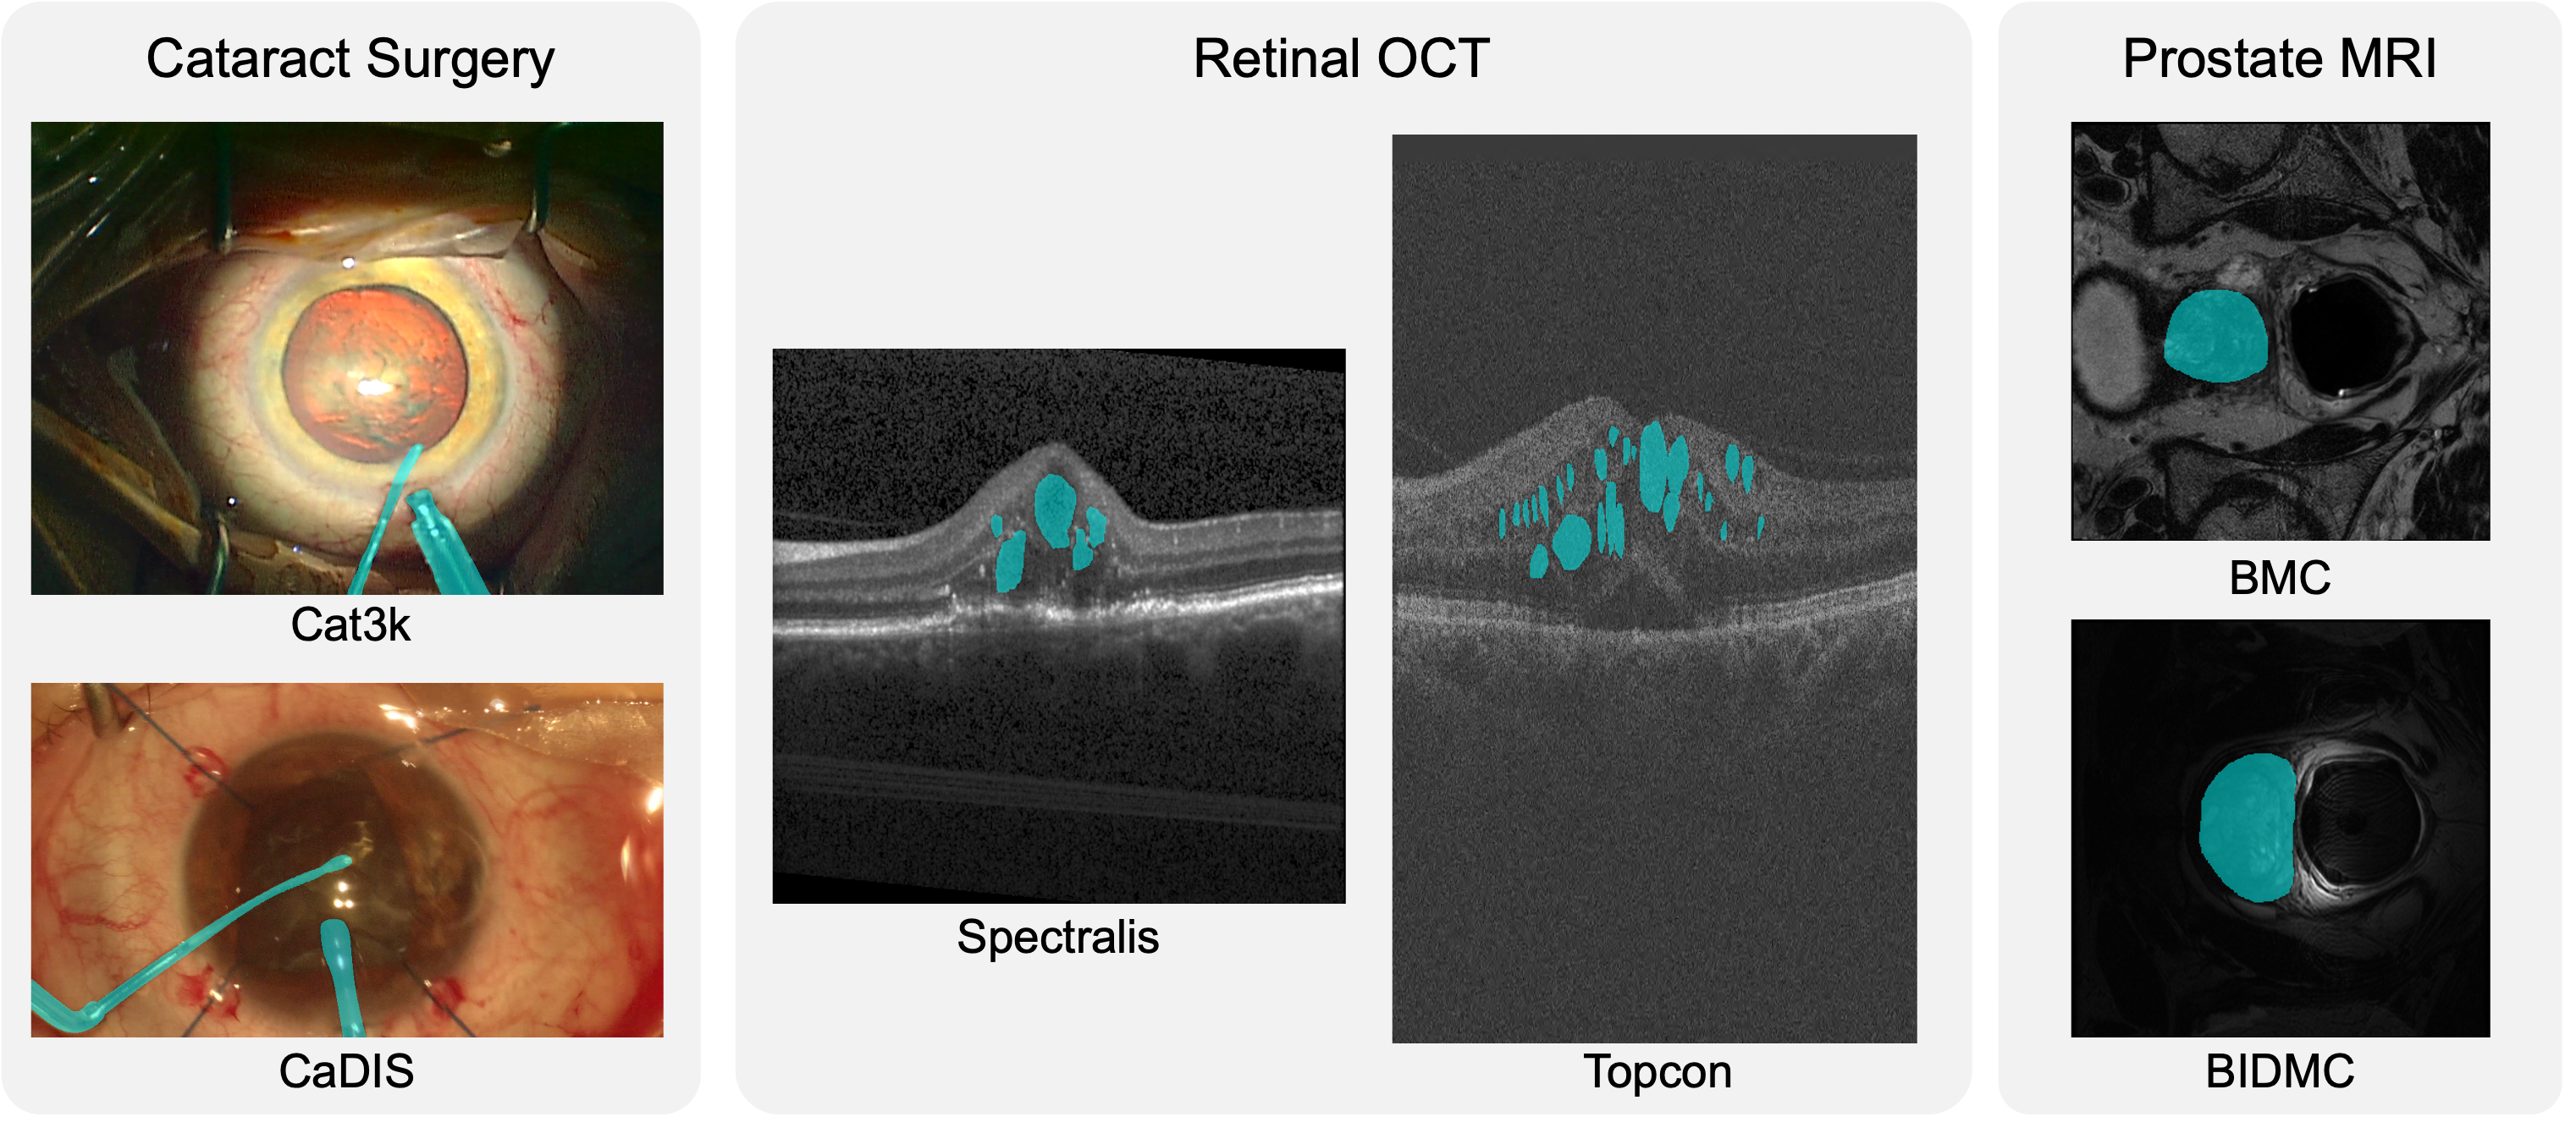
\includegraphics[width=0.95\textwidth]{figures/Datasets2.png}
%\caption{Example images from the three adopted datasets: (1) cross-device-and-center instrument segmentation in cataract surgery videos (Cat101 vs. CaDIS), cross-device fluid segmentation in OCT (Spectralis vs. Topcon), and cross-institution prostate segmentation in MRI (BMC vs. BIDMC).
%}
%\label{fig:datasets}
%\end{figure}